\section{Introdução}

\begin{frame}{Objetivo da Apresentação}
    \begin{itemize}
        \item Demonstrar as principais funcionalidades do \texttt{beamer};
        \item Exibir elementos como listas, figuras, tabelas e equações;
        \item Referenciar bibliografia com Bib\LaTeX{}.
    \end{itemize}
\end{frame}

\section{Listas e Estruturas}

\begin{frame}{Exemplo de Lista Enumerada}
    \begin{enumerate}
        \item Primeiro item;
        \item Segundo item;
        \item Terceiro item.
    \end{enumerate}
\end{frame}

\begin{frame}{Lista em Blocos}
    \begin{block}{Bloco normal}
        Texto de exemplo em bloco.
    \end{block}
    \begin{alertblock}{Bloco de alerta}
        Destaque em vermelho.
    \end{alertblock}
    \begin{exampleblock}{Bloco de exemplo}
        Usado para exemplos práticos.
    \end{exampleblock}
\end{frame}

\section{Figuras e Tabelas}

\begin{frame}{Figura com TikZ}
    \centering
    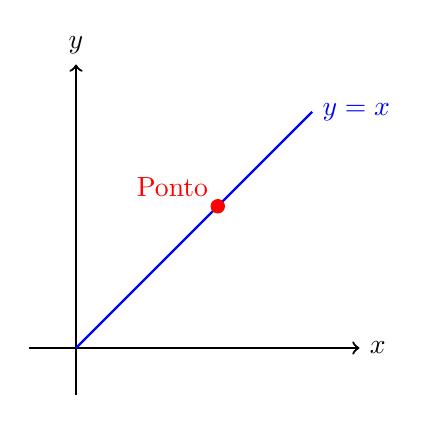
\begin{tikzpicture}[scale=1.2]
        \draw[thick,->] (-0.5,0) -- (3,0) node[right] {$x$};
        \draw[thick,->] (0,-0.5) -- (0,3) node[above] {$y$};
        \draw[blue,thick] (0,0) -- (2.5,2.5) node[right] {$y=x$};
        \filldraw[red] (1.5,1.5) circle (2pt) node[above left] {Ponto};
    \end{tikzpicture}
\end{frame}

\begin{frame}{Tabela de Exemplo}
    \centering
    \begin{tabular}{l|c|c}
        \textbf{Categoria} & \textbf{2024} & \textbf{2025} \\
        \hline
        A & 10 & 12 \\
        B & 20 & 22 \\
        C & 30 & 28 \\
    \end{tabular}
\end{frame}

\section{Equações}

\begin{frame}{Equações Matemáticas}
    Exemplo de equação inline: $y = ax + b$. \\[1em]

    Exemplo destacado:
    \[
        E = mc^2
    \]

    Exemplo de sistema:
    \[
        \begin{cases}
            x + y = 1 \\
            2x - y = 0
        \end{cases}
    \]
\end{frame}

\section{Referências Bibliográficas}

\begin{frame}{Citação no Texto}
    Podemos citar um livro clássico da economia \parencite{smith1776} 
    ou um artigo seminal em ciência de dados \parencite{breiman2001statistical}. 
\end{frame}

\begin{frame}[allowframebreaks]
    \frametitle{Referências}
    \printbibliography
\end{frame}